
This short tutorial presents the most common possible uses of the
BNfinder software. The first part of this tutorial is devoted to
presenting possible options of the software and the input files on
simplistic, synthetic examples. In the second part, we provide more
realistic examples taken from published studies of data for inferring
dynamic and static networks.

In this tutorial, we will assume that you are using the standalone
BNfinder application as downloaded from
\url{http://bioputer.mimuw.edu.pl/software/bnf}, however if you want,
you can also try out these examples with our webserver at
\url{http://bioputer.mimuw.edu.pl/BIAS/BNFinder}.

If you have any questions regarding this document or the described
software, please contact us:
 \url{bartek@mimuw.edu.pl} or \url{dojer@mimuw.edu.pl}
\subsection{Synthetic examples}
\label{sec:simple}
This section shows on several simple networks, how to prepare datasets
and set the parameters for network reconstruction with BNfinder. The
examples include a simple static network, dynamic network and a
network requiring setting prior probabilities.

\subsubsection{Simple static network}
\label{sec:simstat}

\begin{figure}[h]
  \centering
  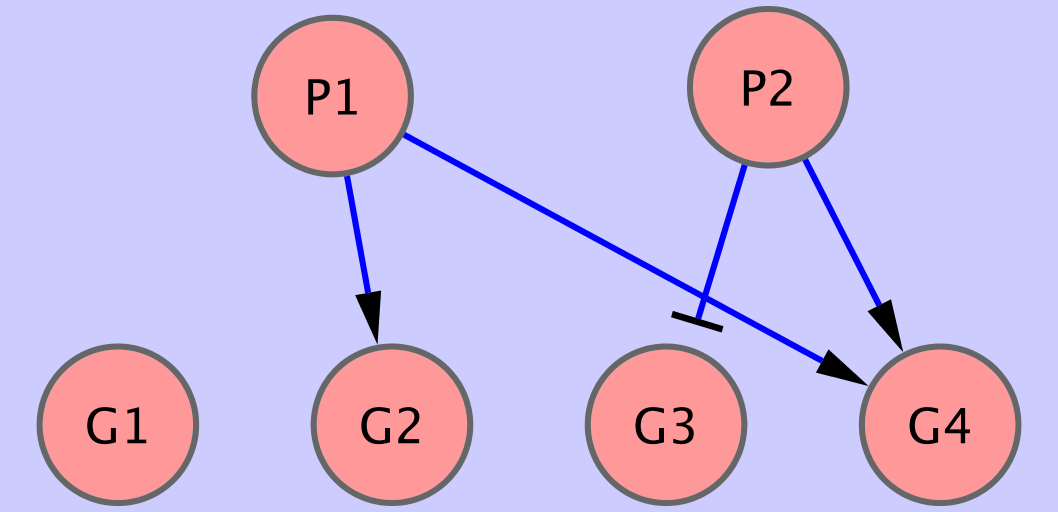
\includegraphics[width=8cm]{img/network1}  
  \caption{Very simple network consisting of 2 regulators and 4 observable regulatees.}
  \label{fig:net1}
\end{figure}

The first example shows how to use BNfinder to learn a simple static
Bayesian network. Let us imagine that we are analysisng cells under
two conditions $P1$ and $P2$ and that we are interested whether any of
the four genes: $G1,G2,G3,G4$ are responding to these conditions. We
assume that the true network is depicted in Fig \ref{fig:net1}, i.e. 
\begin{itemize}
\item $G1$ is not dependent on $P1$ or $P2$,
\item $G2$  is more likely to be expressed under condition $P1$,
\item $G3$ is less  likely to be expressed under condition $P2$,
\item $G4$ is more likely to  be expressed under any of the conditions $P1$ or $P2$.
\end{itemize}

We have collected 100 datapoints from this network, each consisting of
both the state of conditions and the discrete state of expression of
the genes. You can download the input file here \url{data/input1.txt}.

If you open the file in a text editor, please note that the first line
contains the information on the assumed structure:
\begin{verbatim}
#regulators P1 P2
\end{verbatim}
This represents the fact, that we assume that genes ($G1..G4$) can
depend on conditions ($P1,P2$) and not the other way around.

You can try to run BNfinder on this file:
\begin{verbatim}
bnf -e input1.txt -n output1.sif -v
\end{verbatim}
and you will see, that the network topology is reconstructed
properly. Also the orientation of the regulatory interactions is
inferred properly as you can see in the output file
\url{data/output1.sif}.

You can also try to see whether the optimal network is representative
for a larger set of possible suboptimal networks:
\begin{verbatim}
bnf -e input1.txt -n output1w.sif -v -i 4 -t output1.txt
\end{verbatim}
This time, in the output file (\url{data/output1w.sif}), the edge
labels represent the relative weights of different edges. In the file
\url{data/output1.txt}, we can find the originally computed weights
(i.e. relative probabilities -- see manual for details)
for all considered suboptimal sets of parents for all genes.

Instead of fixing the number of returned parents sets 
(option \texttt{-i 4}) you can specify thresholds for their weights
and/or weight ratios to optimal weights.
For example, if you wish to get for each vertex $v$
all parents sets with weights $>\max(0.1,0.01\cdot w_{opt}(v))$, 
where $w_{opt}(v)$ denotes the weight of the optimal parents set of $v$, 
you can type:
\begin{verbatim}
bnf -e input1.txt -n output1a.sif -v -i -1 -m 0.1 -o 0.01 -t output1a.txt
\end{verbatim}

We can also try to analyze the data for this network without
discretization: \url{data/input2.txt}. In this case we need another
directive to indicate that some of the dataseries are continuous:
\begin{verbatim}
#continuous G1 G2 G3 G4
\end{verbatim}

Again if we run BNfinder on this data, 
\begin{verbatim}
bnf -e input2.txt -n output2.sif -v
\end{verbatim}
we can verify, that the output file contains correct information \url{data/output2.sif}.

\subsubsection{Simple dynamic network}
\label{sec:simdyn}

BNfinder can be used also to infer dynamic Bayesian networks from time
series data. In this case it is not necessary to specify the
regulators sets, because DBNs, unlike static networks do not need to
be acyclic.

In the first dataset: \url{data/input3.txt}, we have 1 serie of 20
consecutive measurements of gene expression from gene network depicted
in Fig. \ref{fig:net2}.

\begin{figure}[h]
  \centering
  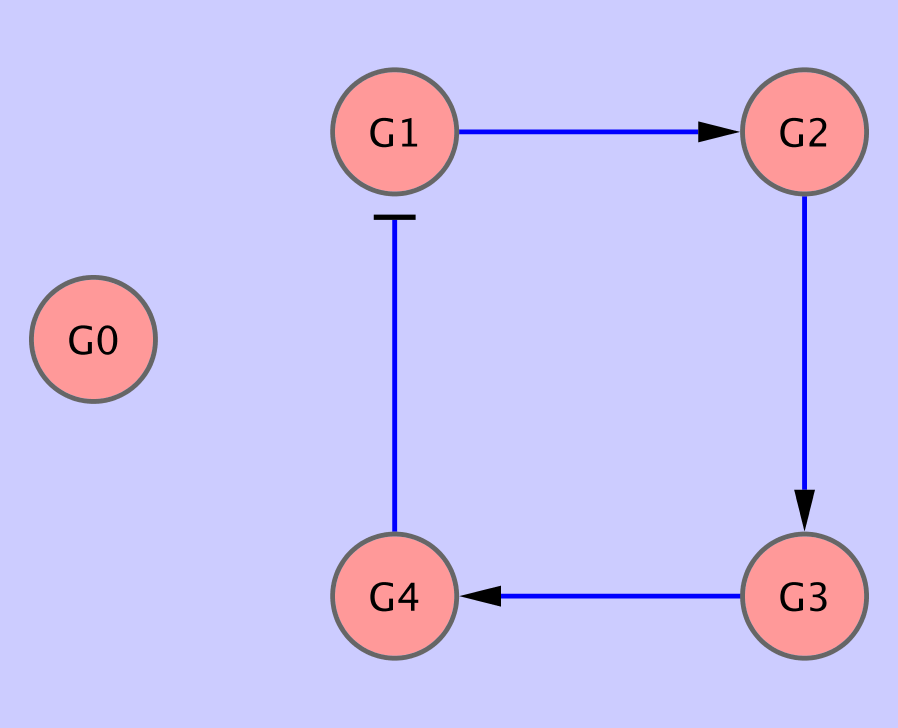
\includegraphics[width=8cm]{img/network2}  
  \caption{Very simple dynamic network consisting of 5 observables}
  \label{fig:net2}
\end{figure}

If we run BNfinder on this data:
\begin{verbatim}
bnf -e input3.txt -n output3.sif -v 
\end{verbatim}
We can see that the program was unable to correctly reconstruct all
the edges. Again, if we look at the statistics of edge occurences in
suboptimal networks,
\begin{verbatim}
bnf -e input3.txt -n output3.sif -v -i 10 -t output3.txt
\end{verbatim}
we can see that the correct edges are the most commonly occuring ones,
but they score lower than empty parent sets.

In this case we can show how perturbational data can be integrated
into this framework. We have collected gene expression from 5
time-series containing one single gene knockout for each of the genes:
\url{data/input4.txt}. The perturbations are noted by including the
following lines in the preamble of the data file:
\begin{verbatim}
#perturbed EXP1 G1
#perturbed EXP2 G2
#perturbed EXP3 G3
#perturbed EXP4 G4
#perturbed EXP5 G0
\end{verbatim}

If we run BNfinder on the perturbed data, we can see that all the edges
are reconstructed with high confidence.
\begin{verbatim}
bnf -e input4.txt -n output4.sif -v -i 10 -t output4.txt
\end{verbatim}

\subsubsection{Setting priors}
\label{sec:simprio}
\begin{figure}[h]
  \centering
  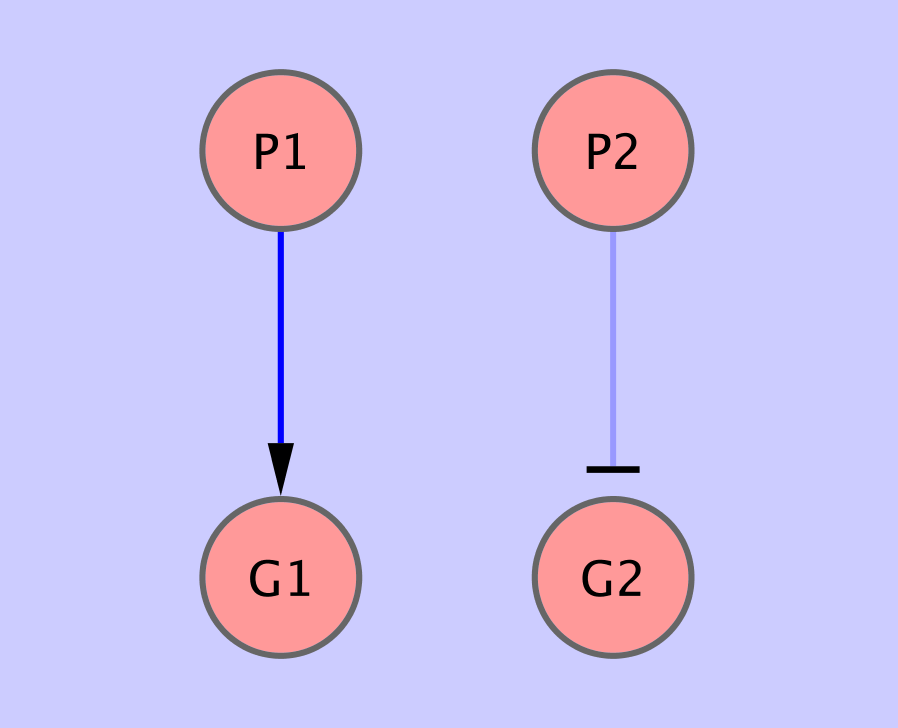
\includegraphics[width=6cm]{img/network3}  
  \caption{Exemplary network containing dependencies of different strength}
  \label{fig:net3}
\end{figure}
In some cases it might be useful to include some prior information on
the network structure into the process of inference. We will
illustrate this on an example of a simple network similar to the one
described in section \ref{sec:simstat}. This time it is an even
simpler network, with 2 conditions and 2 genes as depicted in
Fig. \ref{fig:net3}. Even though topology of the network is very
simple, the problem lies in the fact that the dependence of $G2$ on
$P2$ is weaker than the dependence of $G1$ on $P1$. This is why if we
run our software on the unmodified dataset \url{data/input5.txt}, 
\begin{verbatim}
bnf -e input5.txt -n output5.sif -v  -i 10 -t output5.txt
\end{verbatim}
we can see that the program is unable to recover the $P2\rightarrow G2$
edge. However, if we expect that $G2$ is  responding weakly to its regulators, 
we can increase the prior probability of $G2$ being regulated by any of 
the factors $P1,P2$ via decreasing its weight:
\begin{verbatim}
#prioredge G2 0.33 P2 P1
\end{verbatim}
We can see the edge appearing in the result as expected (see \url{data/input6a.txt}):
\begin{verbatim}
bnf -e input6a.txt -n output6a.sif -v  -i 10 -t output6a.txt
\end{verbatim}

Similarly, if we expect, that in general gene response to condition $P2$ is weaker, we may modify the prior probability of the condition $P2$ to be a regulator:
\begin{verbatim}
#priorvert 0.33 P2 
\end{verbatim}

The result of running BNFinder with this input (\url{data/input6b.txt}) is very similar to the previous one:
\begin{verbatim}
bnf -e input6b.txt -n output6b.sif -v  -i 10 -t output6b.txt
\end{verbatim}

\subsection{Examples of published  datasets}
\label{sec:real}

In this section, we present two more realistic examples of published
datasets used for inference of Bayesian networks. The first one
consists of measurements of states of protein signalling network under
different perturbations \cite{pmid15845847}. It's been used to infer
causal relationships in the form of static Bayesian network.

The second dataset comes from documentation of the Banjo package
\cite{Smith2006} which can be downloaded from
(\url{http://www.cs.duke.edu/$\sim$amink/software/banjo}). It consists
of 2000 observations describing a relatively large dynamic network
consisting of 20 nodes. It may be considered a benchmark of the
efficiency of our algorithm.

The third dataset is converted from an example attached to the
globalMIT software for Bayesian network reconstruction. It is similar
to the second example as it is also generated from a dynamic Bayesian
network and consists of 2000 observations of 20 variables. However, in
this case the variables are much less interconnected and there are
many self-regulatory loops.

\textbf{PLEASE NOTE that these datasets are too large to be run through BNFinder webserver. If you would like to run them, please download the software. }

\subsubsection{Static Protein signalling network}
\label{sec:realStat}

In this section we present how BNfinder can be applied to a protein
signalling network analyzed by Sachs et al \cite{pmid15845847}. We
took the data from the article, and transformed it into the format
suitable for BNfinder. We also needed to specify several properties of
the data in the preamble of the file \url{data/sachs.inp}

\begin{figure}[h]
  \centering
  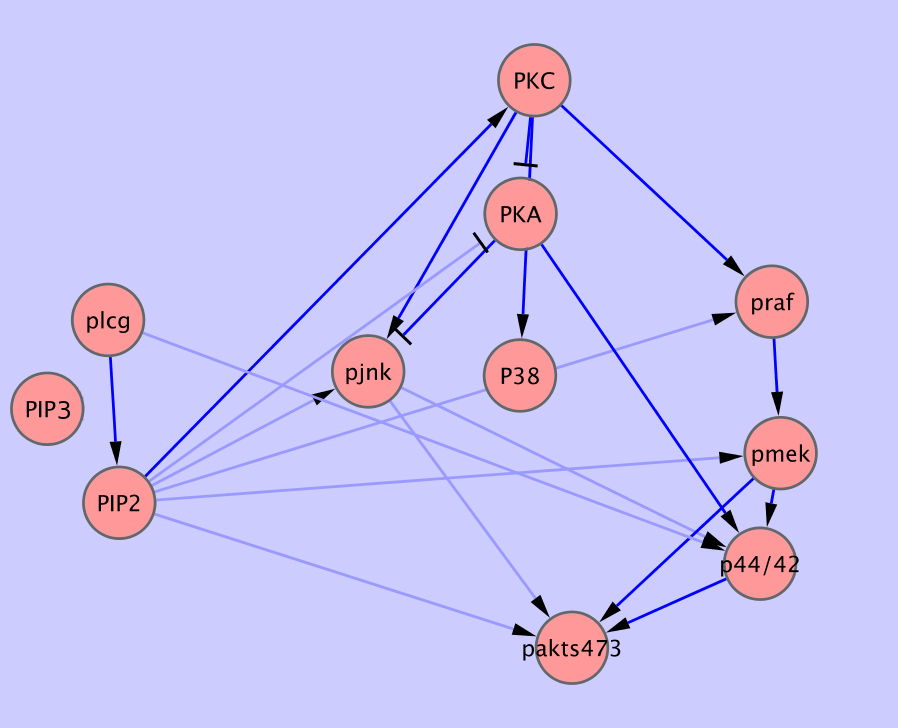
\includegraphics[width=8cm]{img/static}  
  \caption{Reconstruction of the protein signalling network. Dark blue
    arrows represent dependencies found in literature. Light blue
    arrows represent dependencies found by BNfinder but not expected
    by Sachs et al. \cite{pmid15845847}}
  \label{fig:stat}
\end{figure}

Firstly, we needed to specify that the data are continuous measurements:

\begin{verbatim}
#continuous praf pmek plcg PIP2 PIP3 p44/42 pakts473 PKA PKC P38 pjnk
\end{verbatim}

Then, we needed to specify the expected layer structure of the signalling pathway we are studying:
\begin{verbatim}
#regulators plcg
#regulators PIP3
#regulators PIP2
#regulators PKC
#regulators PKA
#regulators praf
#regulators pjnk pmek P38 
#regulators p44/42
#regulators pakts473
\end{verbatim}

Then we needed to specify which of the proteins are affected by different perturbations. 
\begin{verbatim}
#perturbed cd3cd28psitect_0 PIP2
#perturbed cd3cd28psitect_1 PIP2
#perturbed cd3cd28psitect_2 PIP2
...
#perturbed cd3cd28g0076_0 PKC
#perturbed cd3cd28g0076_1 PKC
#perturbed cd3cd28g0076_2 PKC
...
\end{verbatim}

When we finally run the BNfinder:
\begin{verbatim}
bnf -e sachs.inp -n sachs.sif -v 
\end{verbatim}
We obtain the network presented in Fig. \ref{fig:stat}. As we can see,
the topology is quite consistent with the literature data. Out of 17
expected edges, BNfinder recovers 11 correctly. 

\subsubsection{Dynamic Bayesian network}
\label{sec:realDyn}

This is a dataset of substantial size which is used  \cite{bnfinder} to
assess the performance of our inference algorithm. The input dataset
(\url{data/input7.txt}{}) consists of 2000 measurements of 20 variables
and it takes approximately 3 hours to compute it on a modern PC (2.4Ghz
Intel Core 2 duo). 

We can run BNfinder with the following command (note that we are
using the \texttt{-l} option to limit the number of parents to $5$):
\begin{verbatim}
bnf -e input7.txt -n output7.sif -v -l 5 -txt output7.txt
\end{verbatim}

In Fig. \ref{fig:dyn} we can see part of the network reconstructed by
BNfinder. All the edges reported by Banjo are also present in the
optimal network (dark blue). The optimal network contains a number of
additional edges, not reported by Banjo.

\begin{figure}[h]
  \centering
   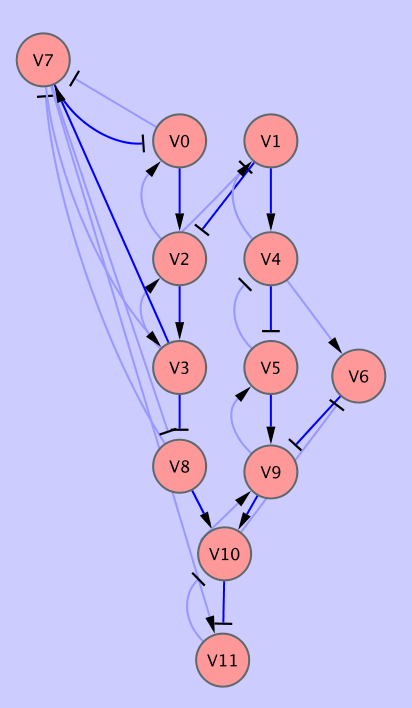
\includegraphics[width=5cm]{img/dynamic}  
  \caption{The optimal network reconstructed by BNfinder from the dynamic benchmark
    dataset. The edges reported also by Banjo are shown in dark blue. }
  \label{fig:dyn}
\end{figure}

If you want to see how much faster the MDL algorithm is, you can also run BNfinder 
with the following command:
\begin{verbatim}
bnf -s MDL -e input7.txt -n output7mdl.sif -v -l 5 -txt output7mdl.txt
\end{verbatim}

\subsubsection{Dynamic network containing self-regulatory loops}
\label{sec:self-loops}

In this example, we can utilize both the \texttt{-g 1} option for
allowing self-regulations as well as the \texttt{-s MIT} option for
using the MIT score.

\begin{verbatim}
bnf -s MIT -e input8.txt -n output8.sif -v -l 3 -txt output8.txt -c output8.cpd -g 1
\end{verbatim}

One additional parameter that is unique to the MIT score is the
significance level $\alpha$ of the $\chi^2$ distribution
(\texttt{-a}). The default level for $\alpha$ is $.9999$, but we can
increase/decrease it if we want to see fewer/more edges respectively.

For example, setting the level alpha to a higher value should give us more edges in the result:

\begin{verbatim}
bnf -s MIT -e input8.txt -n output8.sif -v -l 3 -a .9  -g 1
\end{verbatim}

\subsubsection{Using multiple processors for faster computations}
\label{sec:multicore}

Since most current computers are equipped with multiple processors, we
can take advantage of that fact to speed up BNFinder
computation. Especially for large datasets, such as the ones described
in previous sections, we can take full advantage of the parallell
computation. For example, if we want BNfinder to run on 4 CPUs in
parallell, we can use the \texttt{-k 4} option as in the following example:

\begin{verbatim}
bnf -s MIT -e input8.txt -n output8.sif -v -l 3 -a .9  -g 1 -k 4
\end{verbatim}


\subsection{Example of classification with BNfinder}

\texttt{bnf-cv} and \texttt{bnc} tools can be used to solve classification tasks with classifier based on Bayesian networks. The former is used to perform a cross-validation test and the later to classify a dataset when you already have a classifier. In our example we will try to solve the following problem: we have points within the unit square; our positive set consists of those that are located in top-right and bottom-left corners, i.e. x + y > 1.8 or x + y < 0.2. The training set consists of 100 positive and 100 negative examples. They are visualised in the following Fig. \ref{fig:training}. The data can be downloaded from here (\url{data/training\_set.txt}). We marked x and y as continuous regulators. We will classify only one feature, but it is possible to perform cross-validation and classification procedure for more variables. All variables not marked as regulators are treated as variables to be explained by classifier.

\begin{figure}[h]
  \centering
   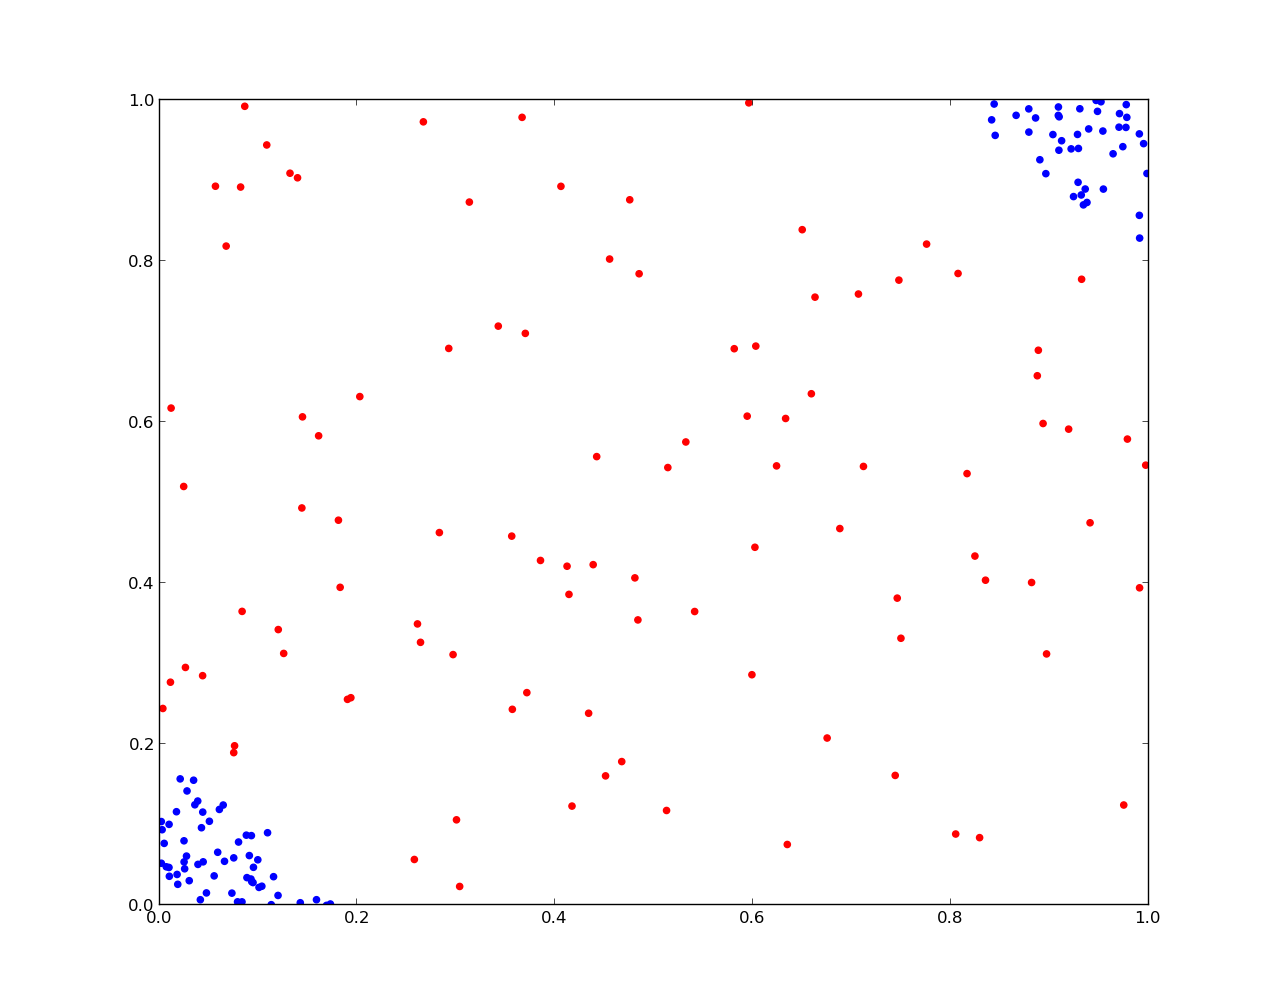
\includegraphics[width=10cm]{img/training}
  \caption{The training set used in the classification example. Positive examples are colored blue. }
  \label{fig:training}
\end{figure}

To perform a 10-fold cross-validation we can use the following command:
\begin{verbatim}
bnf-cv -e training_set.txt -c net.cpd -k 10 -r ROC.pdf
\end{verbatim}

As a result we obtain 10 files (net.cpd0, net.cpd1, ..., net.cpd9) containing networks in cpd format corresponding to respective folds of the cross-validation. Every execution of foregoing command will bring different results, because a split into 10 sets is done randomly. In the result file ROC.pdf there is a ROC plot showing the results of cross-validation (see \ref{fig:ROC}). Further results are printed to the standard output and contains (among others) information about regulators taken to each of 10 classifiers and AUC measure of each classifier's performance. 

\begin{figure}[h!]
  \centering
   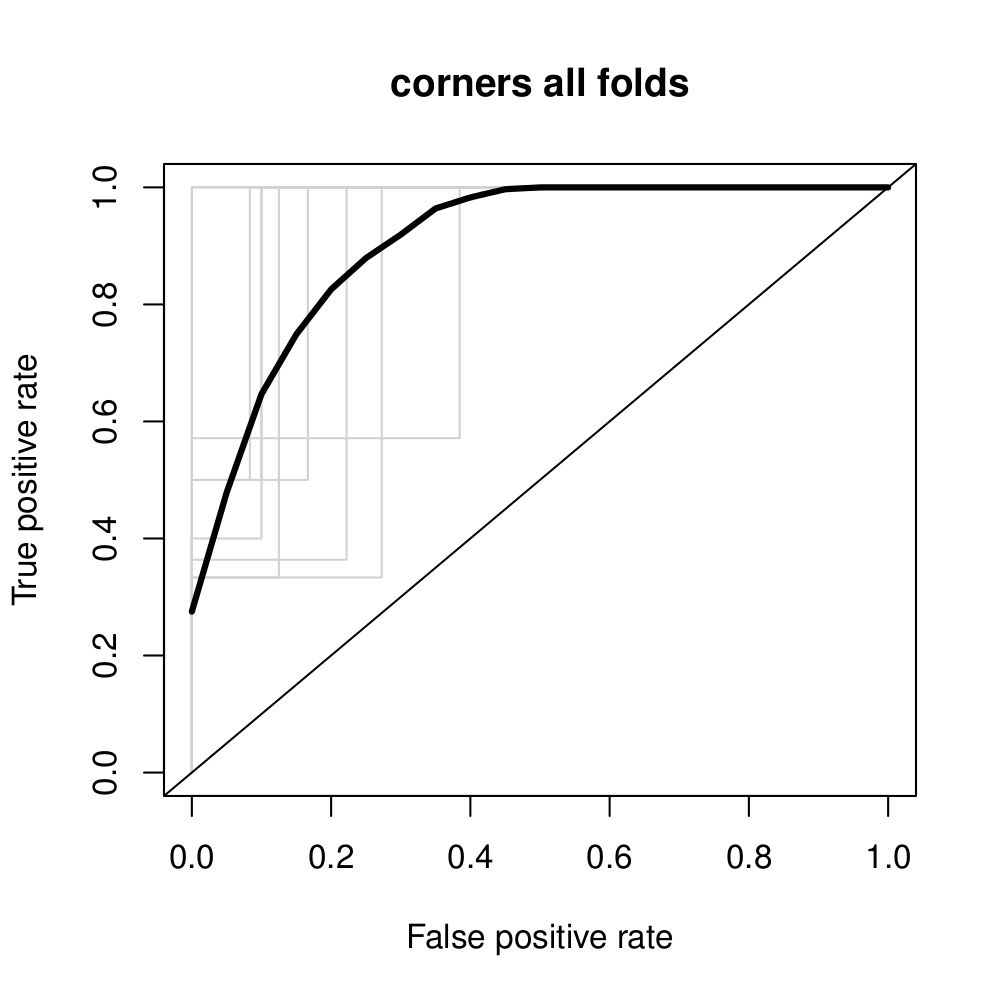
\includegraphics[width=10cm]{img/ROC}
  \caption{The Receiver operating characteristics curve for 10-fold cross-validation. The thick curve shows the average performance of classifiers. }
  \label{fig:ROC}
\end{figure}

To perform classification task on a test dataset we can use any of the nets obtained from cross-validation task but usually it is better to train a classifier on the whole training dataset. It can be done by the following command:
\begin{verbatim}
bnf -e training_set.txt -c net.cpd
\end{verbatim}

We will test out classifier on this (\url{data/test\_set.txt}) dataset which consists of 1000 points from the unit square. Now, by using the \texttt{bnc} tool we can obtain the classification. In the Fig. \ref{fig:classificationresult} we can see the result of classifying our test dataset by classifier in the file net.cpd (we used 0.63 probability threshold to generate the plot):
\begin{verbatim}
bnc -o result.cls -p 1 -c net.cpd -d test_set.txt
\end{verbatim}

\begin{figure}[h!]
  \centering
   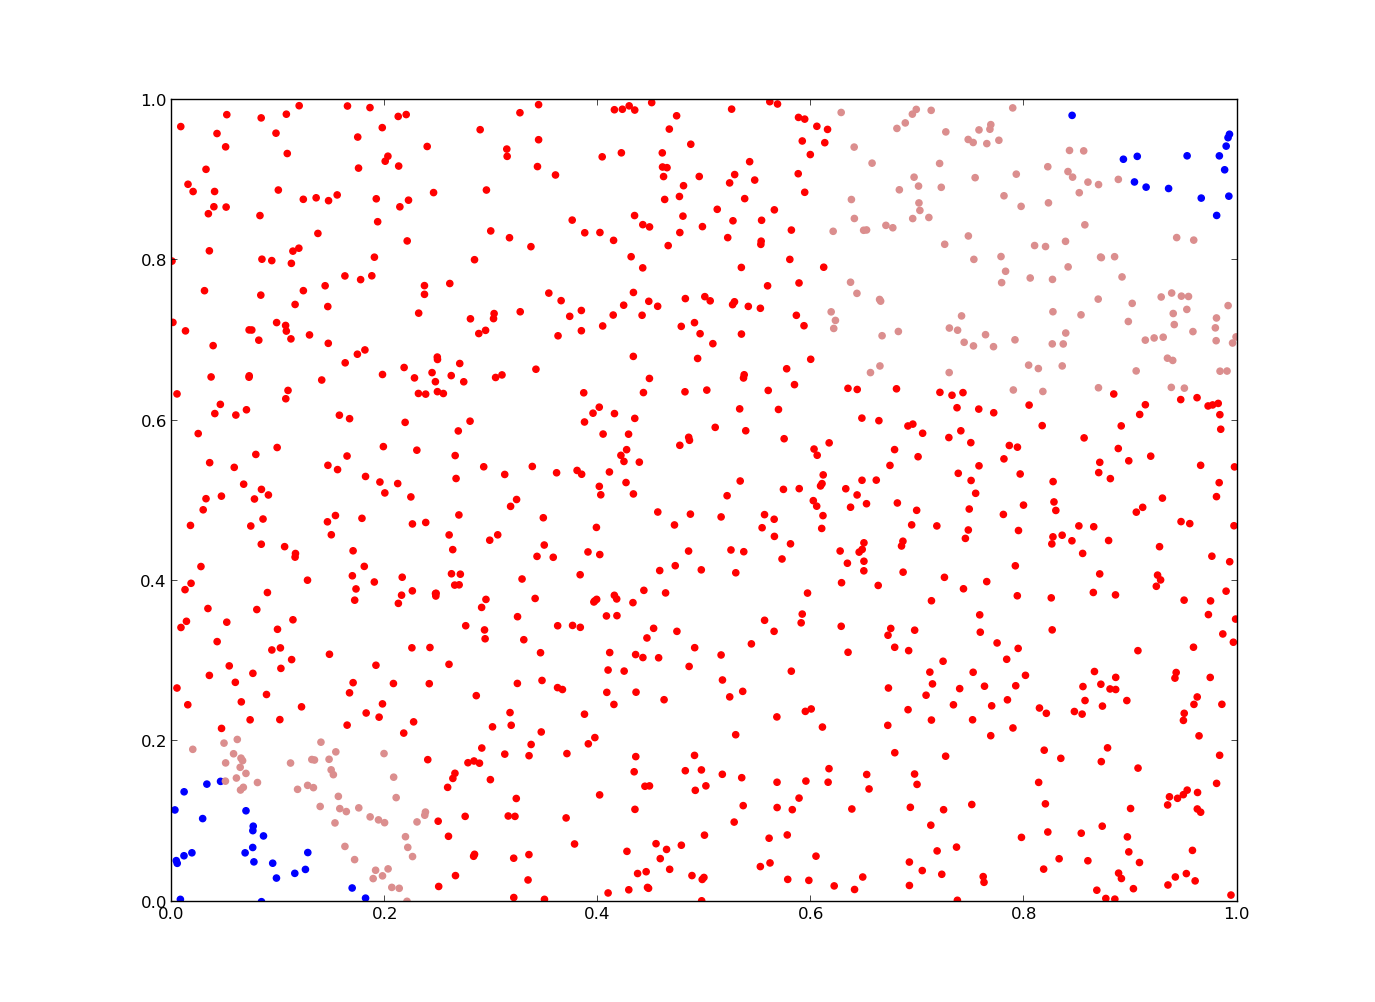
\includegraphics[width=10cm]{img/classificationresult}
  \caption{The result of classification. Blue and red points represent true positives and negatives. There was no false negatives. False positives are colored light red.}
  \label{fig:classificationresult}
\end{figure}

We can also find the most probable class for \texttt{corners} for every experiment by executing:
\begin{verbatim}
bnc -o result.cls -m 1 -c net.cpd -d test_set.txt
\end{verbatim}

Finally, by executing
\begin{verbatim}
bnf-cv -e training_set.txt -k 1 -r ROC.pdf
\end{verbatim}
command one can generate a colored plot of classifier trained on the whole training set. Different colors (explained on the right side of the picture) indicate probability thresholds above which we classify example as a positive one. An example of such a plot can be seen on the Fig. \ref{fig:rock1}.

\begin{figure}[h!]
  \centering
   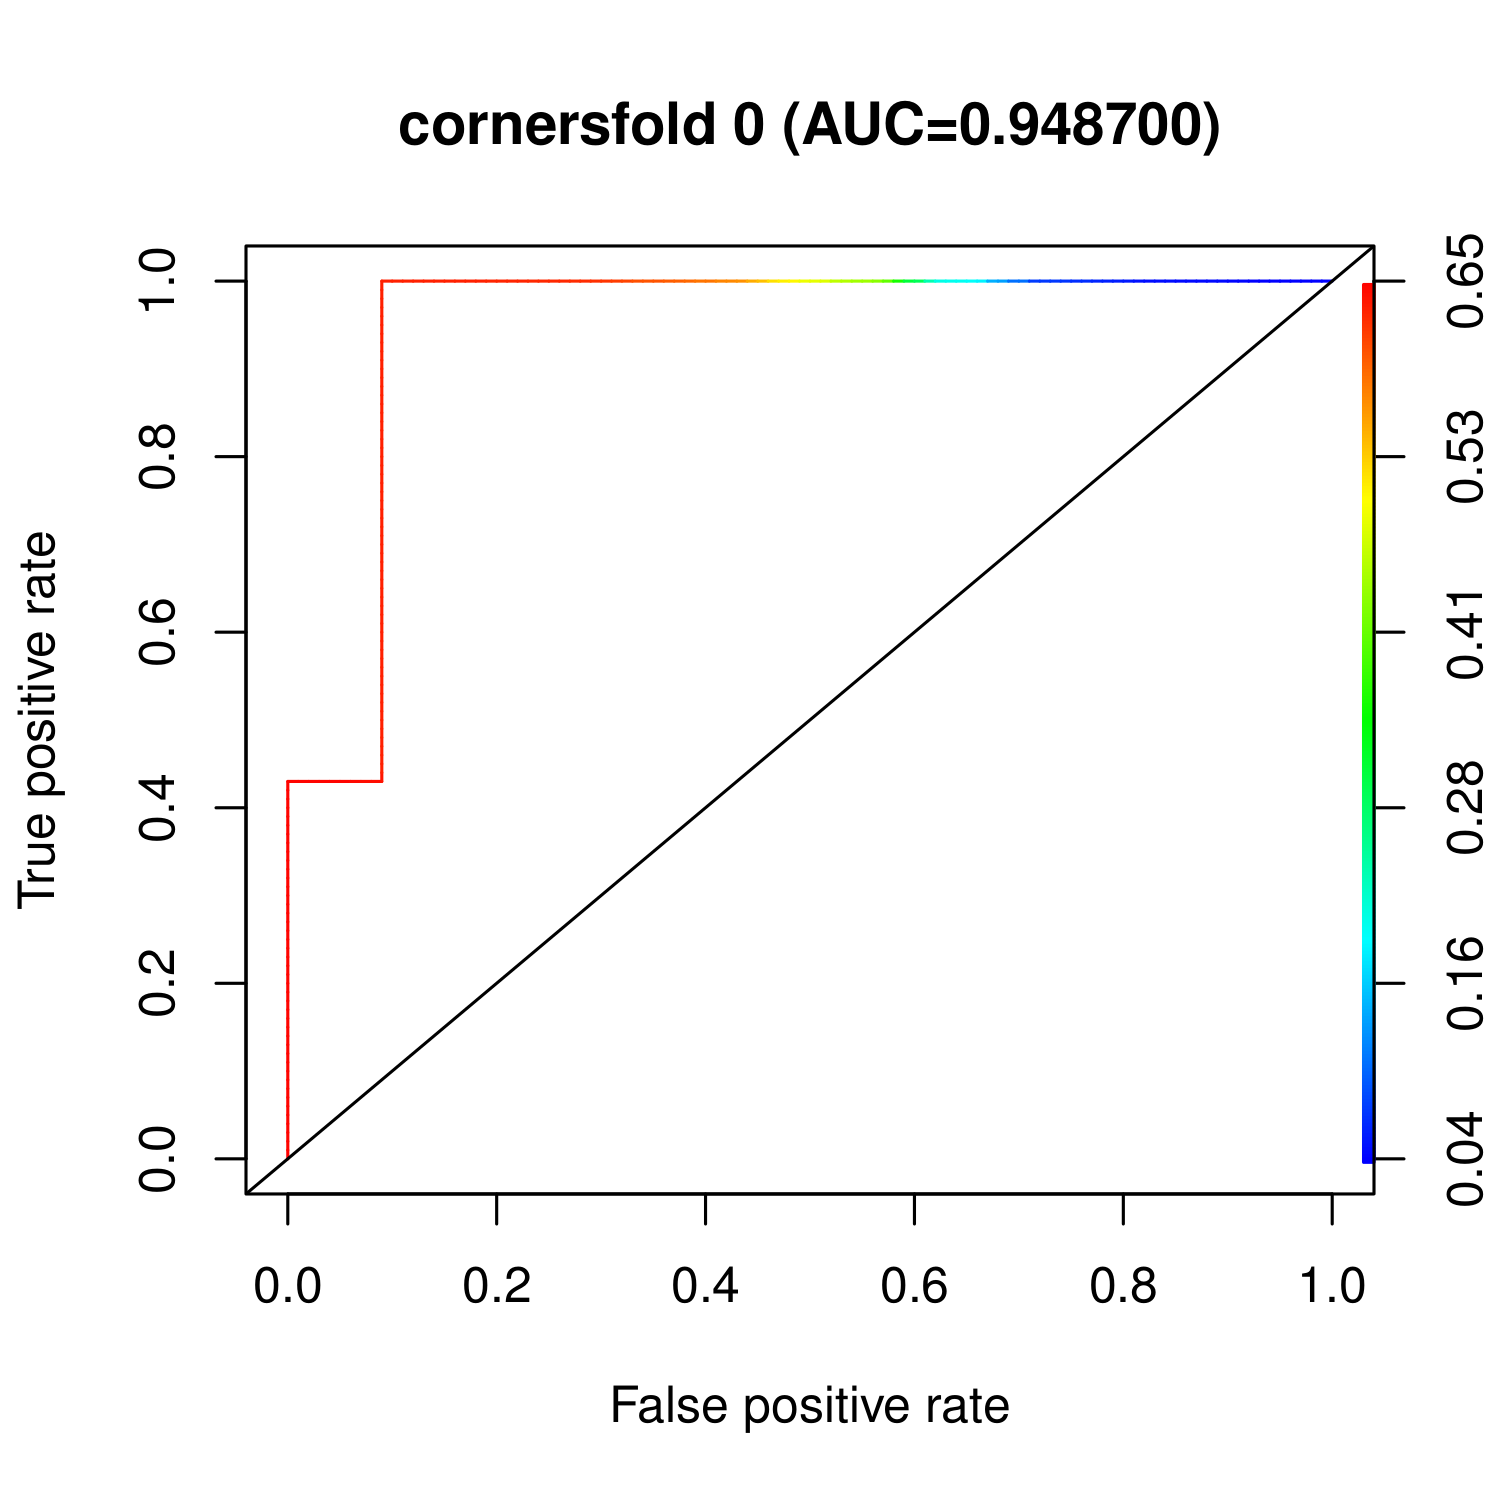
\includegraphics[width=10cm]{img/rock1}
  \caption{The effect of ploting ROC curve from 1-fold cross-validation.}
  \label{fig:rock1}
\end{figure}

%%% Local Variables: 
%%% mode: latex
%%% TeX-master: "tut"
%%% End: 
